\chapter{B1}

{\LARGE 'Provide two charts representing the average bit rate per time unit that crossed the interface or the router in and out during the collecting period.'}

\section{Explicação do código desenvolvido}

A nossa abordagem para este problema foi tentar arranjar uma solução escalável para qualquer tipo de unidades de tempo, dado que para um ficheiro seria uma unidade de tempo de um minuto e outro com 5 segundos. 

Implementamos então duas funções auxiliares para nos ajudar na recolha desta informação. Na figura 7.1 vemos a função \textit{getTimeDiffInSecound(start, to)} onde dado um tempo inicial (start) e um tempo final (to), a função calcula a diferença em segundos desses tempos. 

A função seguinte \textit{getTimeFrameInSecound(file)} recebe um nome de um ficheiro e devolve a unidade de tempo, em segundos, que se pretende. Com esta arquitectura podemos acrescentar livremente novos ficheiros ou mesmo modificar os tempos de cada ficheiro sem ter que se modificar o código base da função b1. O resultado desta função é guardado na variável \textit{timeFrame}.

\begin{figure}[h!]
    \label{high}
    \centering
    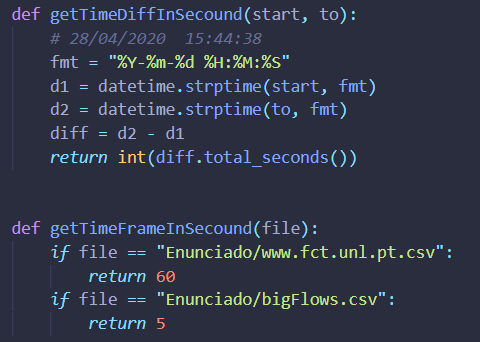
\includegraphics[width=0.6\textwidth]{Images/b1/auxFunctions.png}
    \caption{\textit{Funções auxiliares de b1}}
\end{figure}

Passando agora à explicação do código base da recolha de informação dos ficheiros, começamos por verificar o para cada tuplo (linha) o seu \textit{start\_time\_} (a variável \textit{end\_time\_} não é utilizada), que é o tempo inicial do fluxo que se encontra na primeira coluna dos ficheiros. Posteriormente incializamos a variavel \textit{start\_time} (diferente de \textit{start\_time\_}) que será o tempo inicial do primeiro bloco de tempo a ser analizado. 

A partir dai comparamos esse resultado ao \textit{start\_time\_} de cada fluxo de modo a saber se já passou o tempo necessário para passar para o próximo bloco de tempo. Quando isso acontecer, passamos ao próximo bloco de tempo (counter += 1) e dizemos que agora o \textit{start\_time} agora é o \textit{start\_time\_} do primeiro fluxo do próximo bloco de tempo.

Durante cada bloco inicializamos a nossa estrutura de dados sempre que necessário e adicionamos a ela a informação necessária caso (como requerido pelo enunciado) os IP's sejam externos, utilizando a função \textit{isExternalAddress(file, address)} já explicada nos capítulos anteriores.

\begin{figure}[h!]
    \label{high}
    \centering
    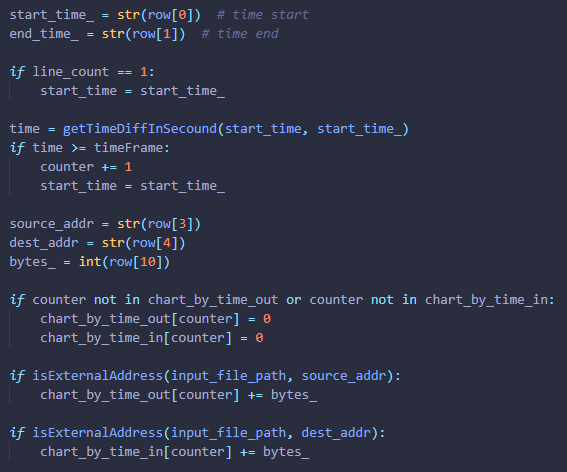
\includegraphics[width=0.9\textwidth]{Images/b1/b1.png}
    \caption{\textit{Código do tópico b1}}
\end{figure}

%----------------------------------------------------------------------------
%----------------------------------------------------------------------------
\newpage

\section{Resultados obtidos pelo ficheiro www.fct.unl.pt.csv}

Os resultados seguintes são o \textit{output} do \textit{byte rate} IN e OUT proposto por intervalos de tempo. Onde o tempo 0 para o ficheiro www.fct.unl.pt.csv equivale ao intervalo de tempo 2020-04-28 14:42:57 -> 2020-04-28 14:43:57 e o tempo 55 (último) equivale ao intervalo de tempo 28/04/2020 15:43:40 -> 28/04/2020 15:44:40, equivalente aos períodos do ficheiro.

\begin{figure}[h!]
    \label{high}
    \centering
    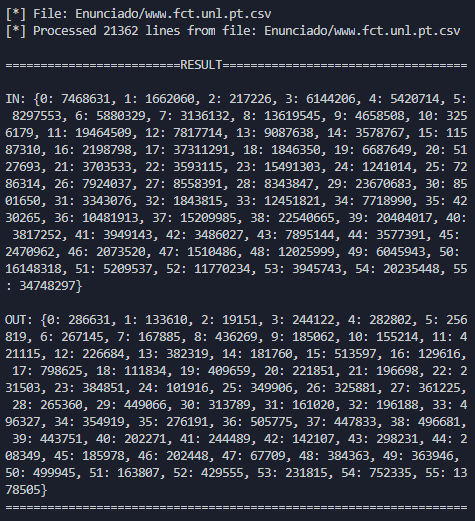
\includegraphics[width=1\textwidth]{Images/b1/b1_a.png}
    \caption{\textit{Output do script b1.py}}
\end{figure}

Utilizando a biblioteca \textit{matplotlib} \cite{MAT} foi-nos possível e tempo de execução do código mostrar um gráfico visual dos dados da figura 7.3.

\begin{figure}[h!]
    \label{high}
    \centering
    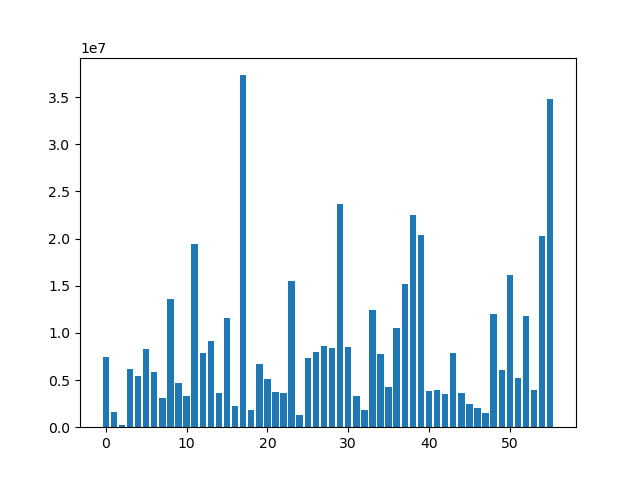
\includegraphics[width=0.9\textwidth]{Images/b1/b1_1.png}
    \caption{\textit{Gráfico do fluxo médio de bytes de entrada}}
\end{figure}

\begin{figure}[h!]
    \label{high}
    \centering
    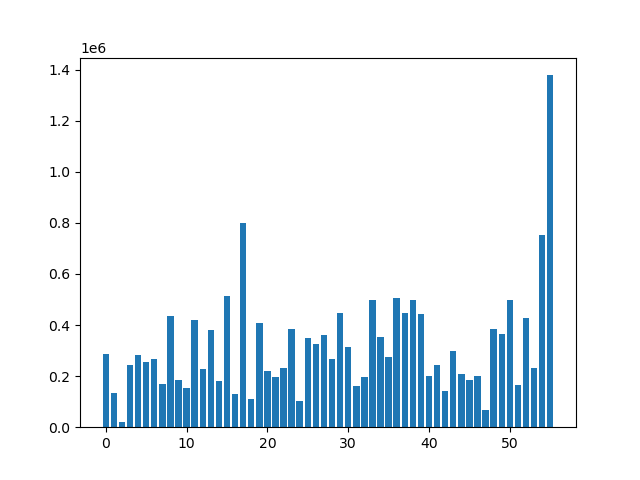
\includegraphics[width=0.9\textwidth]{Images/b1/b1_2.png}
    \caption{\textit{Gráfico do fluxo médio de bytes de saída}}
\end{figure}

\newpage

\section{Resultados obtidos pelo ficheiro bigFlows.csv}

Os resultados seguintes são o \textit{output} do \textit{byte rate} IN e OUT proposto por intervalos de tempo. Onde o tempo 0 para o ficheiro bigFlows.csv equivale ao intervalo de tempo 26/03/2020 20:27:35 -> 26/03/2020 20:27:40 e o tempo 56 (último) equivale ao intervalo de tempo 26/03/2020 20:32:30 -> 26/03/2020 20:32:35, equivalente aos períodos do ficheiro.

\begin{figure}[h!]
    \label{high}
    \centering
    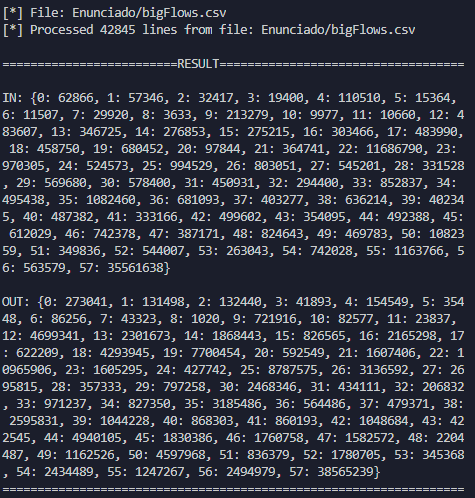
\includegraphics[width=1\textwidth]{Images/b1/b1_b.png}
    \caption{\textit{Output do script b1.py}}
\end{figure}

Utilizando a biblioteca \textit{matplotlib} \cite{MAT} foi-nos possível e tempo de execução do código mostrar um gráfico visual dos dados da figura 7.6.

\begin{figure}[h!]
    \label{high}
    \centering
    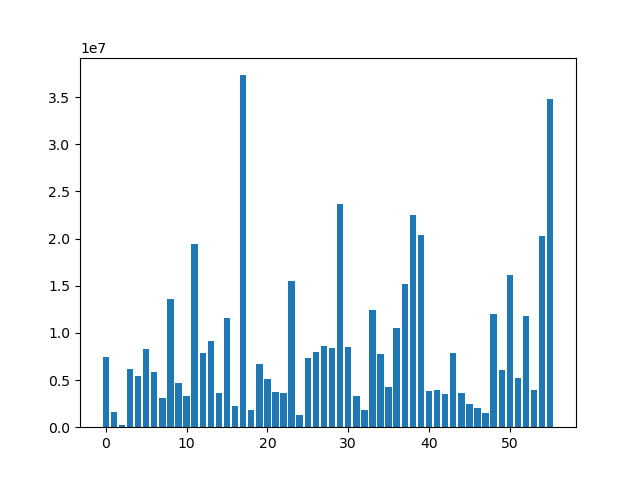
\includegraphics[width=0.9\textwidth]{Images/b1/b1_1.png}
    \caption{\textit{Gráfico do fluxo médio de bytes de entrada}}
\end{figure}

\begin{figure}[h!]
    \label{high}
    \centering
    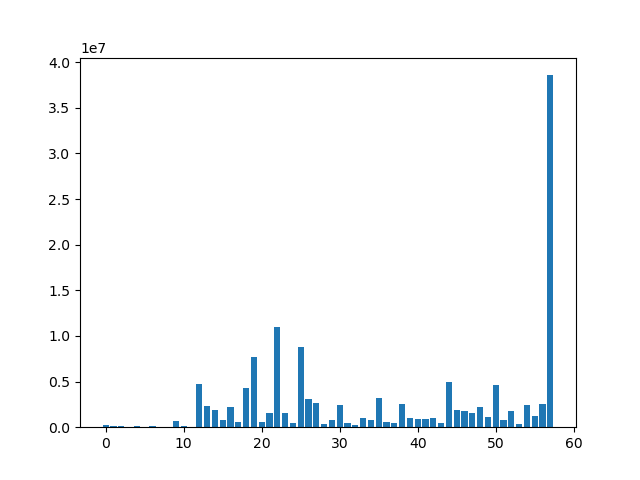
\includegraphics[width=0.9\textwidth]{Images/b1/b1_4.png}
    \caption{\textit{Gráfico do fluxo médio de bytes de saída}}
\end{figure}
